The CISE community served by this proposed infrastructure is composed of three segments: researchers and SLR authors, SLR tool builders, and professional software engineers (see Figure~\ref{figure-ResearchEnabled} for more details).

\begin{figure}
	\centering
	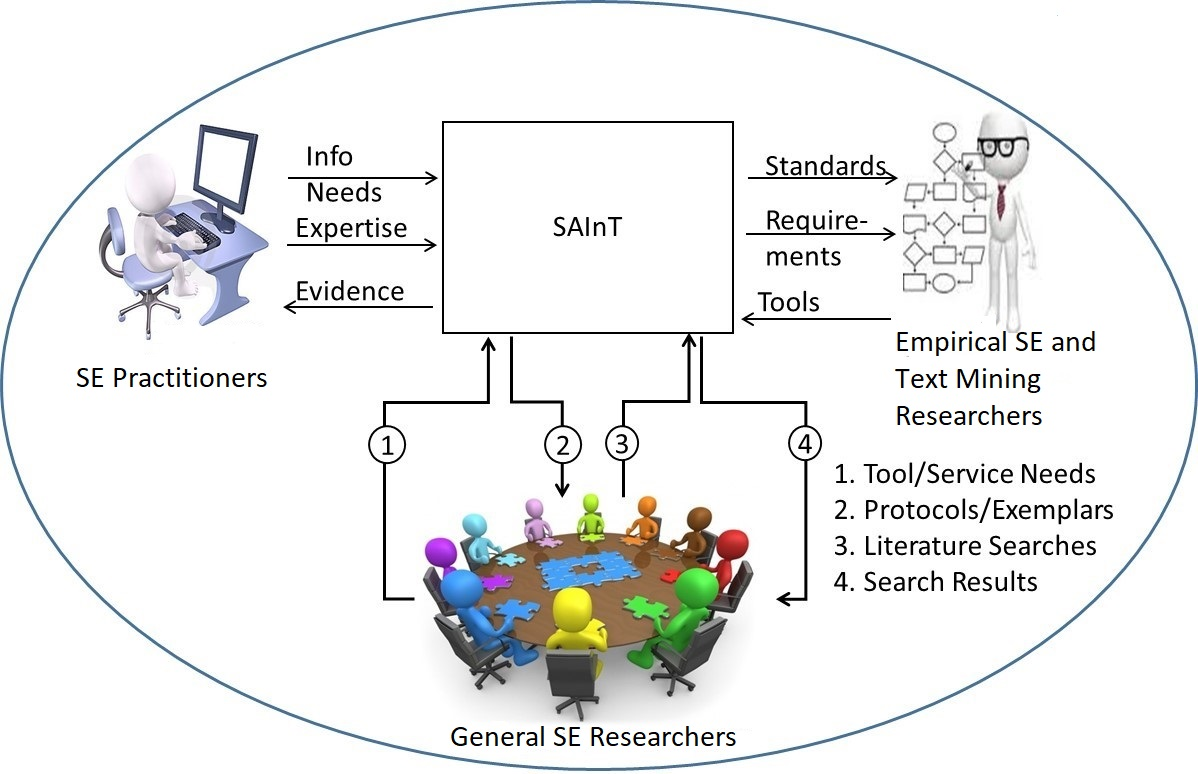
\includegraphics[width=4.5in]{ResearchEnabled}
	\caption{Research Enabled}
	\label{figure-ResearchEnabled}
\end{figure}

\paragraph{Researchers and SLR Authors}
Over 400 unique researchers have published over 300 SLRs in the SE literature.
This portion of the community consists primarily of two groups: expert researchers summarizing the literature about a topic and PhD students working with their advisor as a precursor to dissertation research.
There is no way to identify how many researchers have performed (or partially performed) SLRs that were either not published or incorporated only into PhD students' dissertations (i.e. not published in their own right).
Therefore, the size of the community is potentially much larger than these 400 authors.

%We gathered information about the needs of this portion of the community in two ways.
%First, we surveyed the authors of published SLRs (resulting in 59 responses)~\cite{Carver-etal:13}.
%Second, we conducted two international workshops to gather information about barriers and requirements for SLRs~\cite{Hassler-etal:14,Hassler-etal:16} (Section~\ref{sec:overview:workshops} and~\ref{sec:results:workshops}).
%The results of these surveys and workshops indicated that executing an SLR is a time-consuming, difficult task which is fraught with barriers.

\paragraph{SLR Tool Developers}
While analyzing the existing SLR tools (Section~\ref{sub:existing:tools}), we interacted with the authors of all of the primary SLR support tools: PEx, ReVis, SLuRP, StArt, SLRTOOL, SLR-Tool, and Parsifal.
While each of these tools addresses a portion of the SLR infrastructure needs, there are still gaps (see Section~\ref{sub:existing:tools}).
We will ensure that SAInT provides the necessary APIs and data interchange mechanisms to allow these (and other yet to be developed) tools to individually support portions of the SLR process and collectively support the entire SLR process.
A number of these tool builders have committed to work with us to ensure the flexibility and usefulness of the infrastructure (see attached letters).

\paragraph{Software Engineers} 
In addition to the benefits to researchers described above, the numerous consumers that utilize the results of SLRs will also benefit from the work.  
Practitioners and executives in industry utilize SLR results to identify best practices and to guide decision making.  
Industrial software engineers will benefit from more applied and relevant research that they can commission.
Discussions with the executives (CIOs, VPs, and Consulting Partners the Fortune 500 and the public sector) partnering with the Computer Science and Management Information Systems programs confirm this observation.   
Furthermore, nine of these corporate partners representing 10,000 professional software engineers developing and deploying system across the financial, manufacturing, healthcare, retail and governmental sectors of the economy have provided a letter in support of the development of SAInT (see attached letter).